\subsubsubsection*{EfficientPS}

EfficientPS é uma solução para a segmentação panóptica proposta no artigo \space\citeonline{mohan2020efficientps}, o trabalho apresenta uma arquitetura que se inicia com um backbone — parte para identificar características — usando uma Rede de Pirâmide de Características(RPC)\footnote{Estrutura de pirâmide para extrair características em várias escalas de uma imagem \space\cite{piramide}} de 2 caminhos seguido de dois cabeçotes paralelos um para uma arquitetura de segmentação semântica que é autoria deles e outra de instância com modificações baseadas na topologia Mask R-CNN e finalmente a saída dos dois cabeçotes são combinadas no módulo de fusão panóptica para gerar a saída final com a imagem de segmentação panóptica, esta arquitetura é ilustrada na \cref{fig:arqEP}.

\begin{figure}[ht]
	\caption{Arquitetura geral do EfficientPS}
	\centering % para centralizarmos a figura
	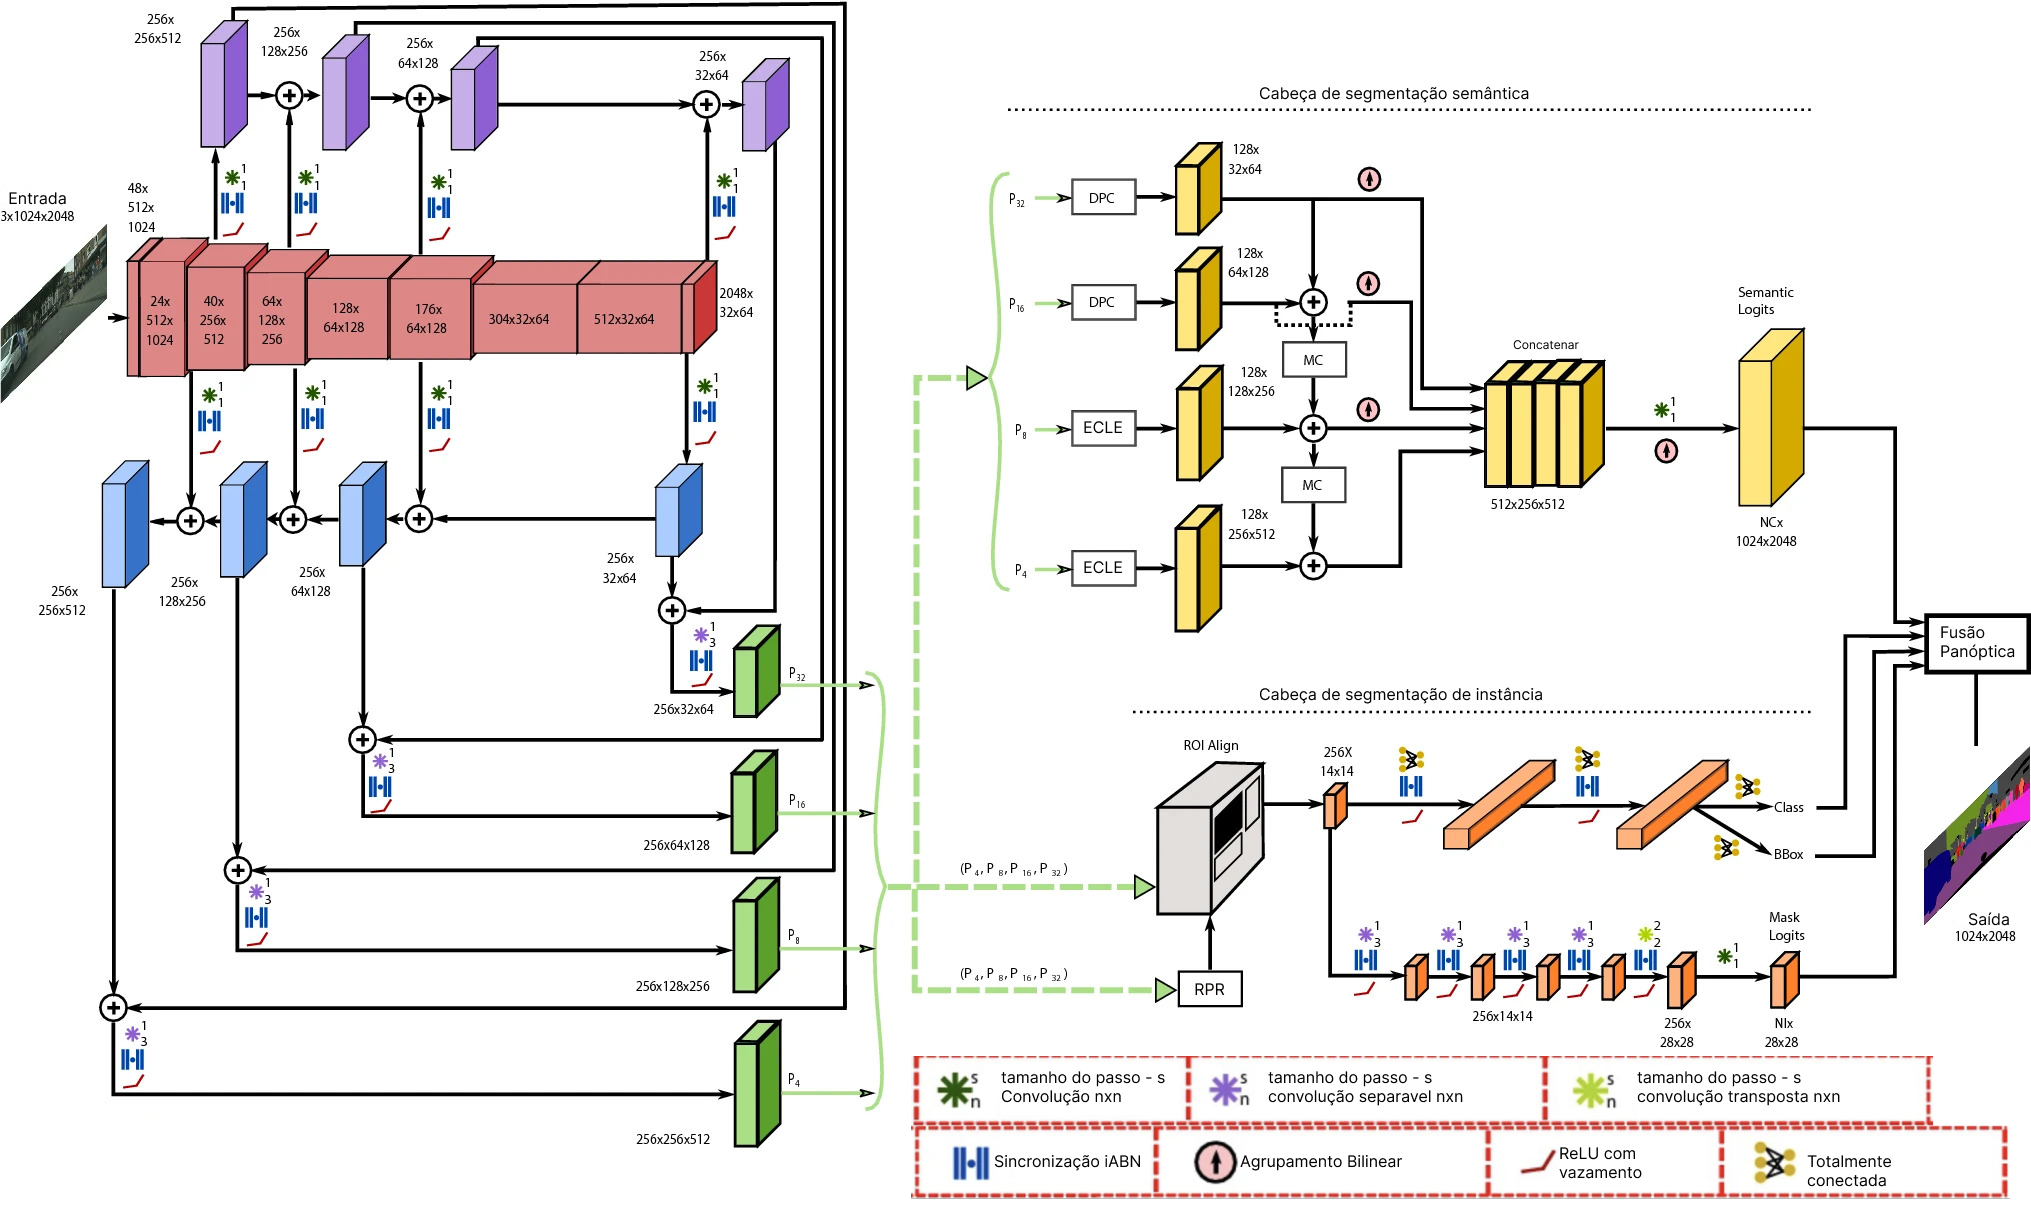
\includegraphics[width=15cm]{figures/arqEP.png} % leia abaixo
	\legend{Fonte: \space\citeonline{mohan2020efficientps}}
	\label{fig:arqEP}
\end{figure}

\subsubsubsection*{Backbone da rede}

A espinha dorsal — ou backbone — se consiste em uma codificação combinado a uma bifurcação paralela usando RPC. O codificador é essencial para arquiteturas de segmentação e para melhorar a capacidade de representação é necessário aumentar o número de parâmetros e a complexidade, porém nesse artigo os autores chegaram numa solução balanceada nesse quesito. O codificador contém nove blocos (em vermelho), mostrado na \cref{fig:arqEP} e a 2º, 3º, 5º e 9º saídas — da esquerda para diretira — correspondem aos fatores de redução de amostragem x4,x8,x16 e x32 respectivamente. Essas saídas vão conectar com a bifurcação paralela que são de sentidos opostos para gerar mais detecções de características. Após isso será feita uma combinação entre camadas de mesma dimensão utilizando camadas de convolução separável em profundidade — divide em etapa espacial e de canal, aplicada a cada canal e cada pixel de saída respectivamente — resultando nas saídas $ P_4 + P_8 + P_{16} + P_{32} $\cite{mohan2020efficientps, redes-neurais-convolucionais-separaveis-em-profundidade}.

\subsubsubsection*{Cabeçote de Segmentação Semântica}

O cabeçote de segmentação semântica é autoria dos autores e é dividido em três módulos sendo eles: Extrator de Características em Larga Escala (ECLE) — ou Large Scale Feature Extractor (LSFE) — para capturar recursos finos em larga escala de forma eficiente, módulo DPC deve ser capaz de capturar contexto de longo alcance, porém em pequena escala e o módulo MC deve ser capaz de mitigar a incompatibilidade entre recursos de grande e pequena escala nas camadas de agregação \space\cite{mohan2020efficientps}.

As quatro entradas do cabeçote $ P_4 + P_8 + P_{16} + P_{32} $ são separadas, sendo $ P_{16} + P_{32} $ — pequena escala — alimentam dois módulos DPC paralelos e $ P_4 + P_8 $ — larga escala — alimentam dois módulos ECLE paralelos \space\cite{mohan2020efficientps}.

\subsubsubsection*{Cabeçote de segmentação de instância}

Este cabeçote é derivada da arquitetura Mask R-CNN e as modificações foram três, sendo: trocar a convolução padrão por convolução separável em profundidade — para reduzir o número de parâmetros consumidos pela rede —, camada de normalização em lote foi substituída por iABN Sync\footnote{normalização em lotes entre cores de GPU para aumentar o desempenho} e a função ReLU definida em \cref{eq:relu_func} por Leaky ReLU definida em \cref{eq:relu_leaky_func} \space\cite{mohan2020efficientps,redes-neurais-convolucionais-separaveis-em-profundidade, serp-ai}.

\subsubsubsection*{Módulo de fusão panóptica}

O módulo da fusão panóptica é necessário para construir a imagem com segmentação panóptica. Nessa parte os resultados são unidos aos dois cabeçotes anteriormente explicados. Esta tarefa não é simples pois é necessário criar uma lógica para obter o melhor resultado diante das sobreposições encontradas. O módulo foi criado no intuito de ser adaptativo e usar as duas entradas de forma equivalente \space\cite{mohan2020efficientps}.

Resumindo o módulo aplica algumas técnicas para reduzir o número de instâncias baseando-se na métrica logist — valor numérico que pontua confiança — aplica algumas agregações entre os resultados dos dois cabeçotes e desenha com fundo preto as instâncias com melhor classificação de confiança, logo depois preenche com a parte de stuff — classes semânticas sem importância — da entrada semântica \space\cite{mohan2020efficientps}.